\documentclass{article}
\usepackage[utf8]{inputenc}
\usepackage{textcomp}
\usepackage{gensymb}
\usepackage{graphicx}
\usepackage{multicol}
\usepackage{amsmath}
\usepackage{amssymb}
\usepackage{physics}
\usepackage{hyperref}
\usepackage{cancel}

\graphicspath{ {./chap2images/} }

\oddsidemargin=-.3in
\evensidemargin=-.5in
\textwidth=7in
\topmargin=-1in
\textheight=10in

\parindent=.2in
\pagestyle{plain}

\title{\textbf{Fractions!} \\ \large Math 1 - Chapter 2}
\author{Theo Rode}
\date{}

\begin{document}

\maketitle

Maybe you have seen fractions before, maybe you haven't, and either is okay. But either way, lets start at the beginning: what is a fraction? Well, if you look up the definition of a fraction, and use the non-math answer, you find:
\begin{center}
    ``Fraction: a small or tiny part, amount, or proportion of something.''
\end{center}

So what does this suggest? Well the definition would indicate that a \textit{fraction} is something that is a ``tiny part'' of something else. So what does that look like? 

\section*{Back to Multiplication}

Let's go back to how we defined multiplication. We initially called it ``super addition,'' but we then moved to thinking about multiplication as adding together a certain number of groups of objects. That means that each of those groups we added together in the multiplication are ``small parts'' of the result. 
For example, if we are looking at $4 \times 5$, we are adding together \textbf{5 groups} of \textbf{4 items}:
\begin{center}
    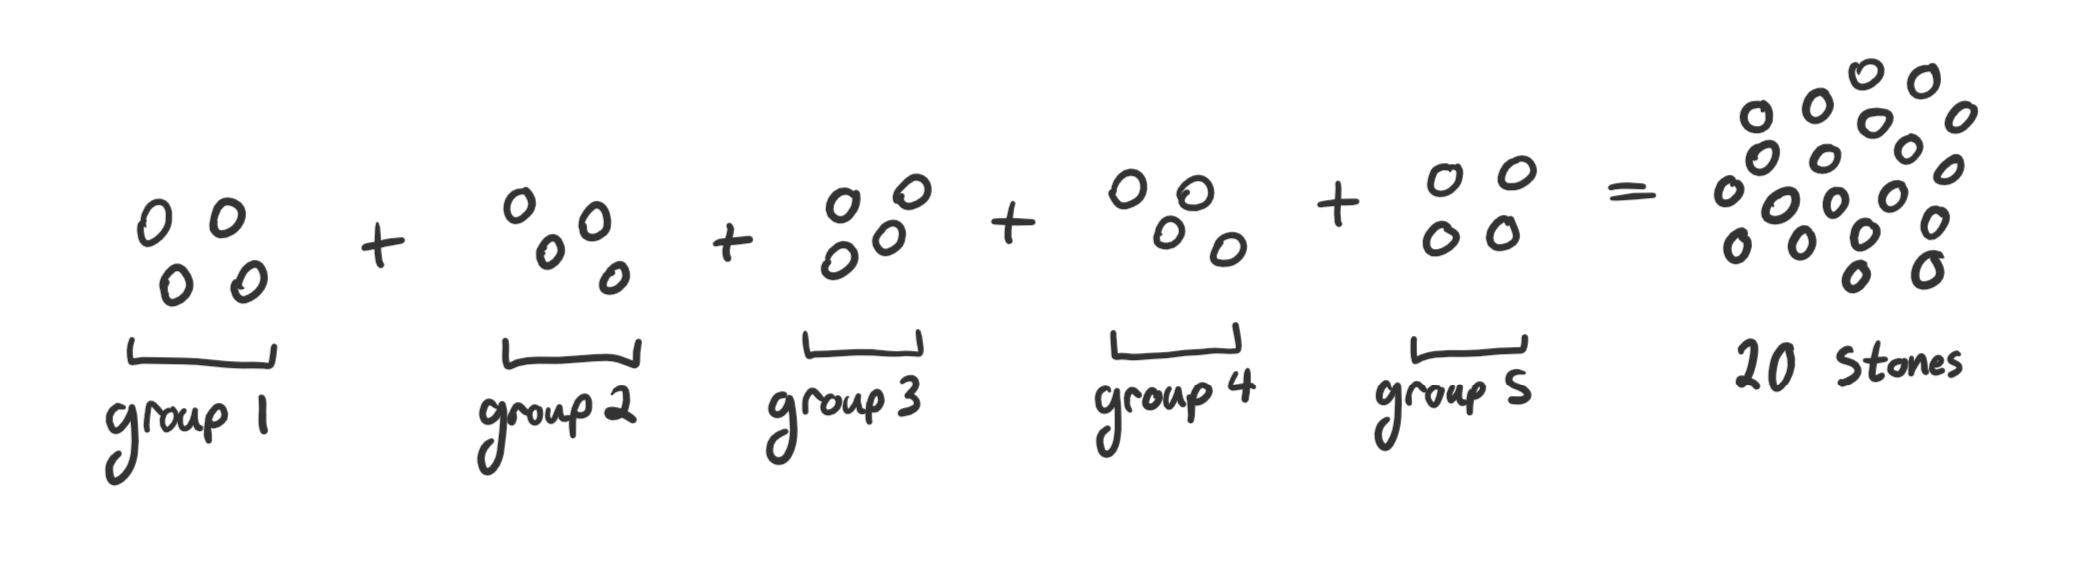
\includegraphics[scale=0.5]{chapter2_draw1.png}
\end{center}
If it takes \textbf{5 groups} of 4 to get to 20 ($4 \times 5 = 20$), then we say that 4 is \textbf{one-fifth} of 20. It takes 5 groups of 4 to add up to 20. 

\section*{And... Back to Fractions...}

So what really is \textbf{one-fifth}? We call it a fraction and if we were to write it with math, we would write:
\[ \frac{1}{5} \]

What this expression is saying is that this is \textbf{one group} of five. In fact, this isn't just a representation of a concept, but a number! And it is a super special number. Why? Well, we say that:
\[ 20 \times \frac{1}{5} = 4 \]

And why is this cool? Well remember: $4 \times 5 = 20$. By multiplying by $\frac{1}{5}$, we \textbf{undo} multiplying by 5! In other words, we have found an inverse for multiplying by 5!

But what does it mean to multiply by a fraction? I have just told you that this is something you can do, but how can you think of this process? Well let's look at a random problem, say:
\[ 15 \times \frac{1}{3} \]

So, for starters, what does $\frac{1}{3}$ mean? Well, much like how we called $\frac{1}{5}$ one-fifth, we call $\frac{1}{3}$ one-third. One third, instead of representing one of five groups, represents \textbf{one of three groups}. 

How can we use this information to solve $15 \times \frac{1}{3}$? Well, we thought of multiplying by $\frac{1}{5}$ as selecting one of the 5 groups that made up 20, this gave us 4. So what if we did this here? We would have to start by splitting 15 into 3 groups. What would these groups be? 

After a little bit of thinking, you may realize that: 
\[ 5 + 5 + 5 = 15 \]

Or in other numbers:
\[ 5 \times 3 = 15 \]

Or in other words: 3 groups of 5 add up to 15! So, to multiply by $\frac{1}{3}$, we want to select one of these three groups. Therefore, we get the result:
\[ 15 \times \frac{1}{3} = 5 \]

Again, we find that multiplying by $\frac{1}{3}$ is ``undoing'' multiplying by 3. If these fractions appear to follow the same rules as the inverse we found for adding (negative numbers), what was the other attribute of the inverse that we found? A number, added to its inverse, gives us the additive identity. In numbers:
\[ 4 + -4 = 0 \]

If you remember from the previous class, the identity for multiplication is 1. Therefore, if we are to believe that these fractions are the multiplicative inverse, we should find this to be true:
\[ 3 \times \frac{1}{3} = 1 \]
\[ 4 \times \frac{1}{4} = 1 \]
\[ 5 \times \frac{1}{5} = 1 \]

I am going to leave you on this thought for now and I want you to think about this all a bit more for homework. 

\section*{Problems}
\begin{multicols*}{2}
    For problems 1-5, draw a picture of the multiplication (counting up stones or whatever you like) and compute the result.
    \begin{enumerate}
        \item $16 \times \frac{1}{4}$
        \item $18 \times \frac{1}{6}$
        \item $8 \times \frac{1}{2}$
        \item $6 \times \frac{1}{3}$
        \item $25 \times \frac{1}{5}$
    \end{enumerate}

    \begin{enumerate}
        \item[6. ] What type of number is $\frac{1}{3}$ or $\frac{1}{5}$? Look back at our previous ``What is an Operation?'' class notes and recall how we defined the following types of numbers: natural numbers, whole numbers, and integers. Do these fractions fit into any of these categories? Are they a completely different type of number? 
        \item[7. ] We can say that 1 is less than 2, in that the number 2 represents more ``things'' than the number 1. While it is less clear why right now, we also define negative numbers to be less than 0. What about fractions? Say the number $\frac{1}{3}$. Is is greater than 0? Is it less than 0? Greater or less than 1? Somewhere else? Talk about why you come to the conclusion you do.
        \item[8. ] What does the value of $\frac{1}{3} + \frac{1}{5}$ mean? Can you calculate it? If you do calculate it, try to add it to some other numbers/multiply it with some other numbers. Do the results you get make sense? 
        \item[9. ] What does the value of $\frac{2}{3}$ mean? Can you multiply this number by another number? Say 3? or 15? What does this value represent? 
        \item[10. ] What does the value of $\frac{1}{4} \times \frac{1}{5}$ mean? Can you calculate it? As a hint: what happens when you calculate $20 \times \frac{1}{4}$ and then multiply what you get from that by $\frac{1}{5}$?
        \item[11. ] What does $2 \times \frac{1}{3}$ mean? What about $2 \times \frac{1}{4}$? 
        \item[12. ] Does the value of $2 \times \frac{1}{4}$ have anything to do with $\frac{1}{2}$? What about $\frac{3}{6}$? Can you draw any conclusions from patterns you find with these numbers?
    \end{enumerate}
\end{multicols*}

\end{document}
